\documentclass[14pt]{extreport}
\usepackage{cmap}
\usepackage[utf8]{inputenc}
\usepackage[english,ukrainian]{babel}
\usepackage{graphicx}
\usepackage{geometry}
\usepackage{listings}
\usepackage{amsmath}
\usepackage{float}
\usepackage{array}
\geometry{
	a4paper,
	left=20mm,
	right=20mm,
	top=20mm,
	bottom=20mm
}
\lstset{
	language=bash,
	tabsize=4,
	breaklines,
	keepspaces,
	showstringspaces=false,
}
\graphicspath{ {./pictures} }
\setlength{\parindent}{4em}

\newcommand\subject{Аналіз вимог до програмного забезпечення}
\newcommand\lecturer{професор кафедри ПЗ\\Грицюк Ю.І.}
\newcommand\teacher{асистент кафедри ПЗ\\Масюкевич В.В.}
\newcommand\mygroup{ПЗ-32}
\newcommand\lab{6}
\newcommand\theme{Візуалізація результатів експертного оцінювання якості
	програмного забезпечення}
\newcommand\purpose{Розроблення методики візуалізації інформації, отриманої
	внаслідок оброблення експертних оцінок якості ПЗ за різними критеріями з
	використанням полярних діаграм}

\begin{document}
\begin{normalsize}
	\begin{titlepage}
		\thispagestyle{empty}
		\begin{center}
			\textbf{МІНІСТЕРСТВО ОСВІТИ І НАУКИ УКРАЇНИ\\
				НАЦІОНАЛЬНИЙ УНІВЕРСИТЕТ "ЛЬВІВСЬКА ПОЛІТЕХНІКА"}
		\end{center}
		\begin{flushright}
			Інститут \textbf{КНІТ}\\
			Кафедра \textbf{ПЗ}
		\end{flushright}
		\vspace{140pt}
		\begin{center}
			\textbf{ЗВІТ}\\
			\vspace{10pt}
			До лабораторної роботи № \lab\\
			\textbf{На тему}: “\textit{\theme}”\\
			\textbf{З дисципліни}: “\subject”
		\end{center}
		\vspace{40pt}
		\begin{flushright}
			
			\textbf{Лектор}:\\
			\lecturer\\
			\vspace{10pt}
			\textbf{Виконав}:\\
			
			студент групи \mygroup\\
			Коваленко Д.М.\\
			\vspace{10pt}
			\textbf{Прийняв}:\\
			
			\teacher\\
			
			\vspace{28pt}
			«\rule{1cm}{0.15mm}» \rule{1.5cm}{0.15mm} 2023 р.\\
			$\sum$ = \rule{1cm}{0.15mm}……………\\
			
		\end{flushright}
		\vspace{\fill}
		\begin{center}
			\textbf{Львів — 2023}
		\end{center}
	\end{titlepage}
		
	\begin{description}
		\item[Тема.] \theme.
		\item[Мета.] \purpose.
	\end{description}

	\section*{Лабораторне завдання}
	\begin{enumerate}
		\item Побудувати табл. 6.4, в яку потрібно занести оцінки експертів за кожним
		критерієм оцінювання якості ПЗ. Стосовно оцінок користувачів, то тут для кожного
		критерію потрібно взяти середні значення, отримані як мінімум від 10 респондентів.
		\item Обчислити за формулою (6.1) усереднені оцінки, отримані від k-го
		експерта за усіма критеріями із врахуванням вагового коефіцієнта i-го критерію.
		\item Обчислити за формулою (6.3) усереднені оцінки, отримані для i-го
		критерію за всіма експертами із врахуванням вагових коефіцієнтів кожного критерію.
		\item Обчислити за формулою (6.2) інтегральну оцінку якості ПЗ від усіх
		експертів, які беруть участь в оцінюванні якості ПЗ.
		\item Обчислити за формулою (6.4) інтегральну оцінку якості ПЗ за всіма
		критеріями оцінювання якості ПЗ.
		\item Побудувати полярні діаграми для усереднених оцінок, отриманих від усіх
		статичних і динамічних експертів, а також для інтегральної оцінки якості ПЗ.
	\end{enumerate}
	
	\begin{figure}[H]
		\centering
		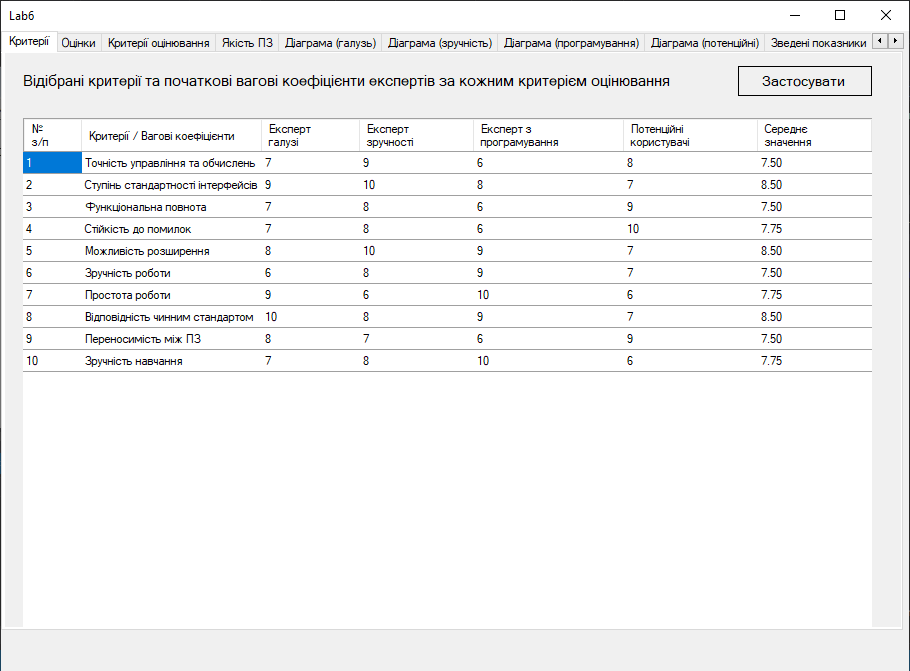
\includegraphics[scale=0.55]{1}
		\caption{Критерії та початкові вагові коефіцієнти експертів за кожним критерієм}
	\end{figure}

\begin{figure}[H]
	\centering
	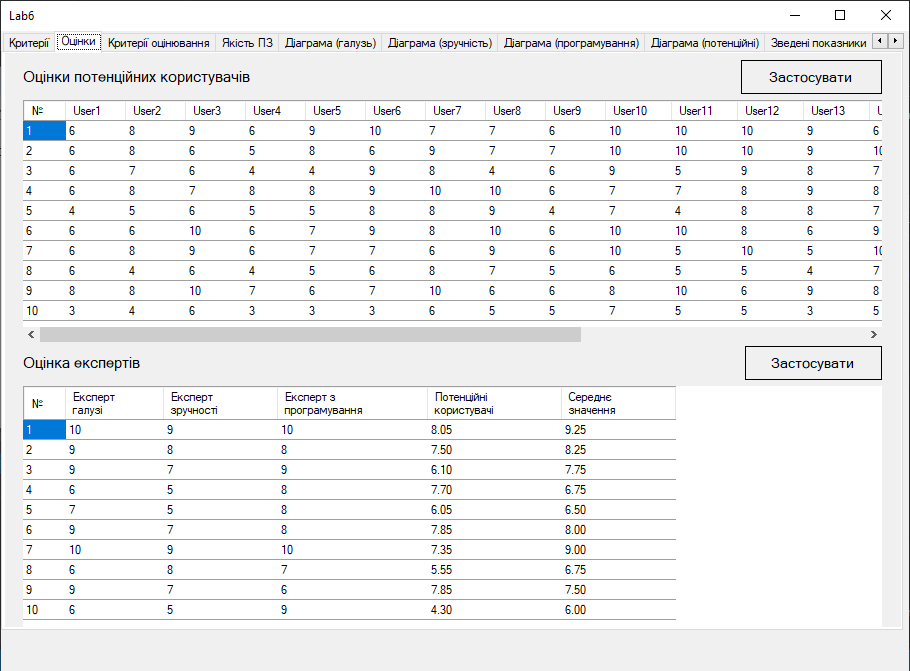
\includegraphics[scale=0.55]{2}
	\caption{Оцінки експертів та оцінки потенційних користувачів}
\end{figure}

\begin{figure}[H]
	\centering
	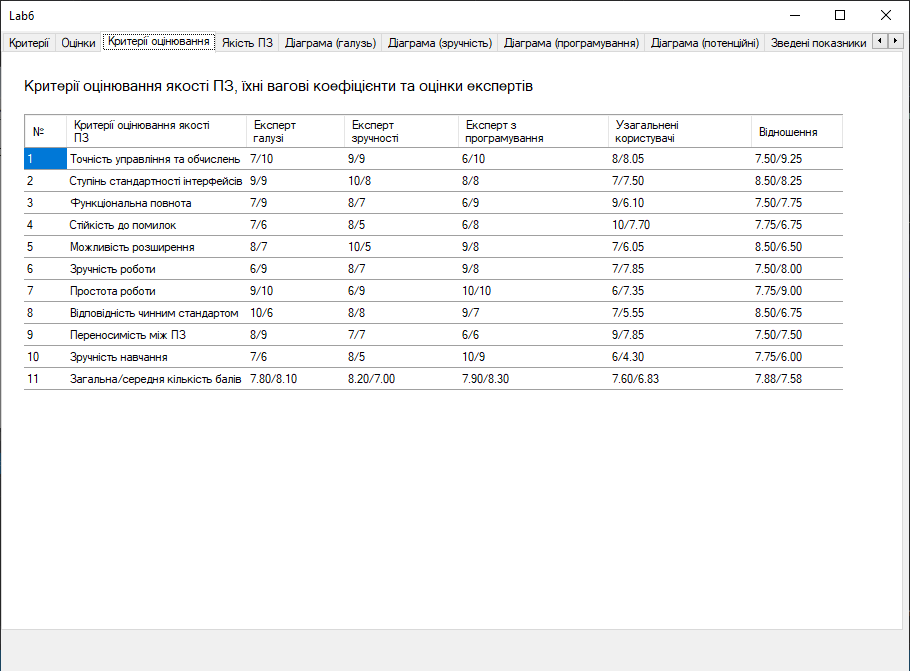
\includegraphics[scale=0.55]{3}
	\caption{Критерії оцінювання якості ПЗ, їхні вагові коефіцієнти та оцінки експертів}
\end{figure}

\begin{figure}[H]
	\centering
	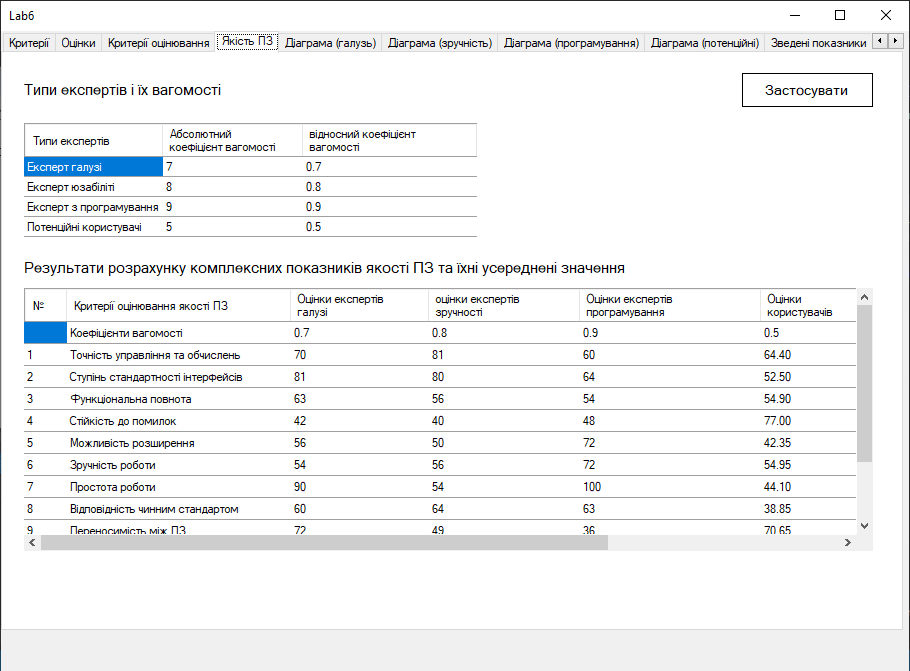
\includegraphics[scale=0.55]{4}
	\caption{Типи експертів і їхні вагомості}
\end{figure}

\begin{figure}[H]
	\centering
	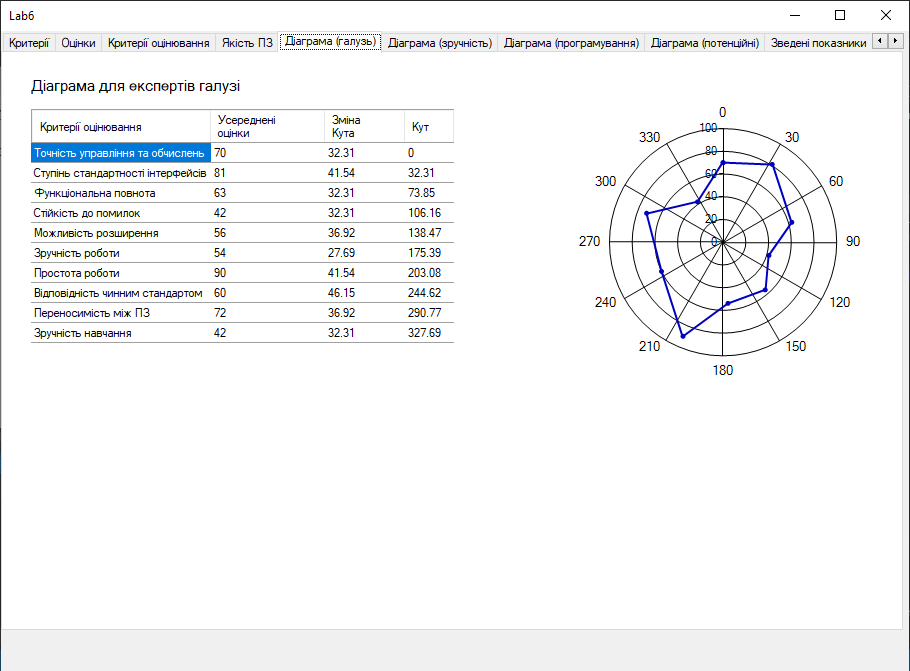
\includegraphics[scale=0.55]{5}
	\caption{Діагарама для екпертів галузі}
\end{figure}

\begin{figure}[H]
	\centering
	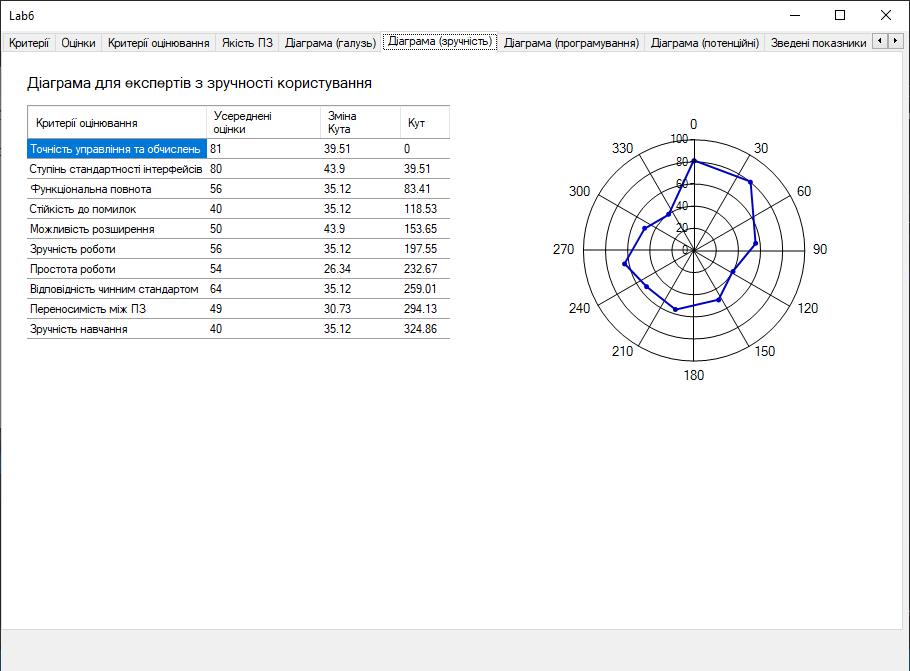
\includegraphics[scale=0.55]{6}
	\caption{Діагарама для екпертів зручності}
\end{figure}

\begin{figure}[H]
	\centering
	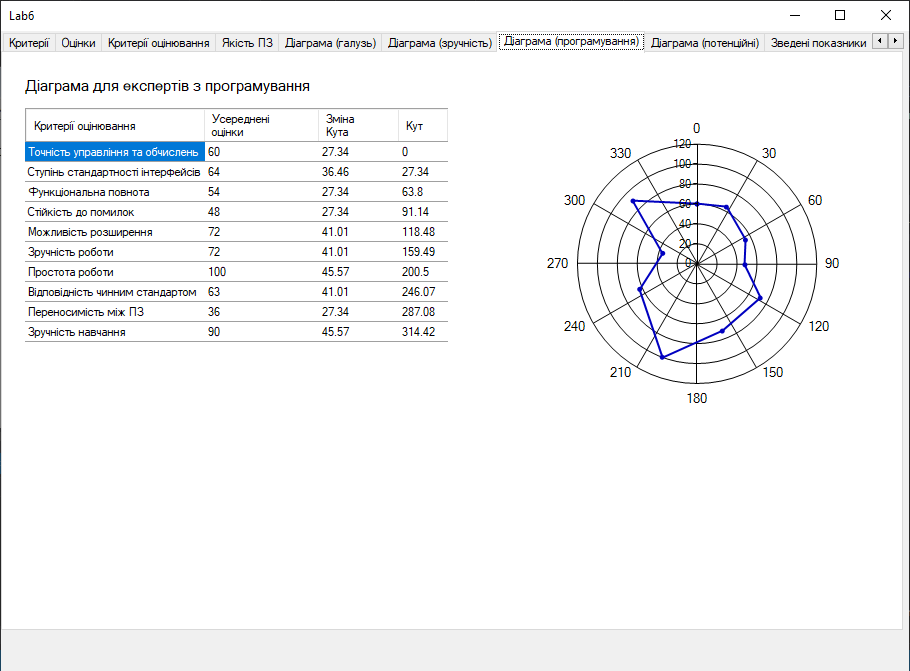
\includegraphics[scale=0.55]{7}
	\caption{Діагарама для екпертів з програмування}
\end{figure}

\begin{figure}[H]
	\centering
	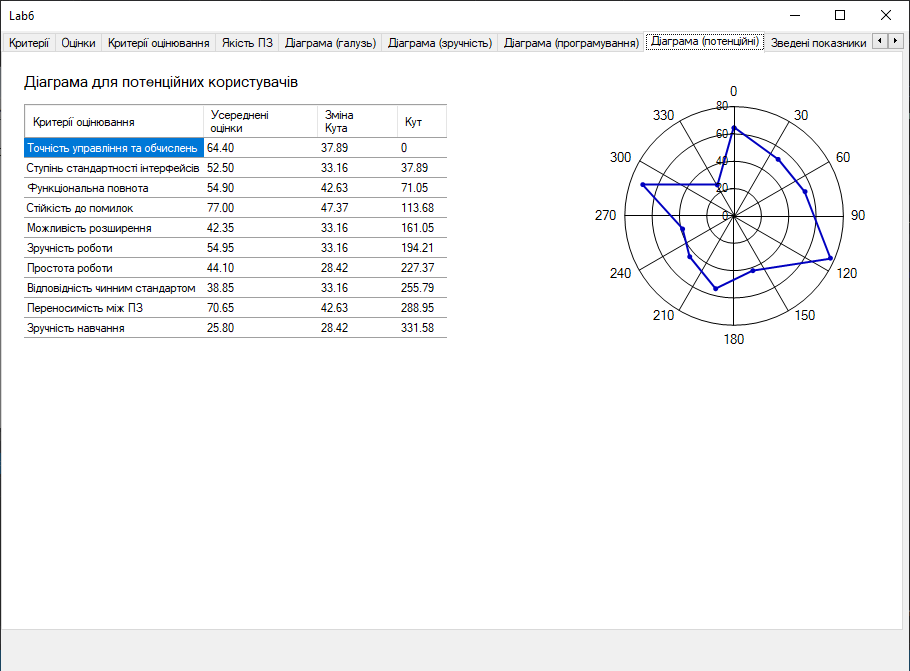
\includegraphics[scale=0.55]{8}
	\caption{Діагарама для потенційних користувачів}
\end{figure}

\begin{figure}[H]
	\centering
	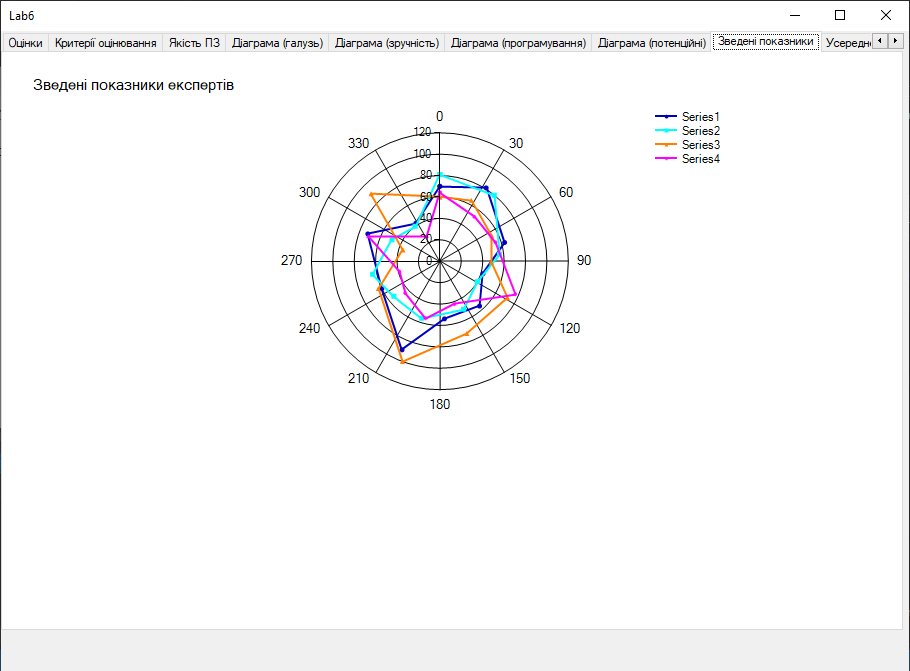
\includegraphics[scale=0.55]{9}
	\caption{Зведені показники екаспертів}
\end{figure}

\begin{figure}[H]
	\centering
	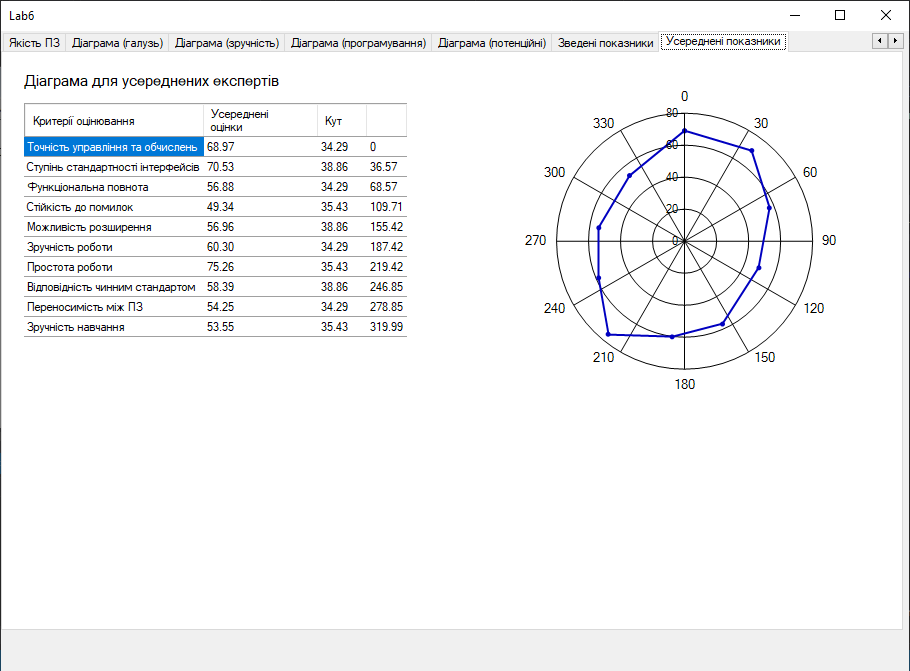
\includegraphics[scale=0.55]{10}
	\caption{Діаграма для усереднених експертів}
\end{figure}

	
	\section*{Висновок}
	Під час виконання лабораторної роботи я розробив методики візуалізації інформації, отриманої
	внаслідок оброблення експертних оцінок якості ПЗ за різними критеріями з
	використанням полярних діаграм.
	
\end{normalsize}
\end{document}
